\scanpage{46}
\mspage{8}
Donc le diagramme squelettique
\[(*)\quad\diagram{\begin{tikzcd}H^\bullet_{\underline D}(U,\xi)\arrow[dr]&&H_{\underline D}(U',\xi)\arrow[dl,no head]\\&H^\bullet_{\underline D}(U\cap U',\xi)&\end{tikzcd}},\]
\inserted{du type $\underline\Psi^{\mathrm{op}}$,} provient-il d'un diagramme \unsure{concret|ouvert}
\[\sigma_0\deleted{\unsure{\xi_0}}\overset{\mathrm{déf}}=\overline\varphi_*(\unsure{a}_{\overline X})\in\underline D(\underline\Psi).\]
Considérons l'inclusion
\[\underline\Psi\overset{\underline k}{\subset}\deleted{\unsure{*}}\Delta^1\times\Delta^1=\diagram{\begin{tikzcd}&(0,1)\arrow[dr,no head]&\\(0,0)\arrow[ur,no head]\arrow[dr]&&(1,1)\\&(1,0)\arrow[ur]&\end{tikzcd}}\]
déduite de $\Psi$ en lui rajoutant l'élément final manquant $(1,1)$. Soit $\underline k$ l'inclusion, et considérons le ``carré cartésien''
\[\sigma=\underline k_*(\sigma_0)\in\underline D(\Delta^1\times\Delta^1)\]
\deleted{Donc les fibres de $\sigma$ en les points de}
On a
\[\underline k^*(\sigma)\simeq\sigma_0,\]
donc le \deleted{\unsure{fibré diagramme}} squell. induit par $\sigma$ sur $\Psi$ n'est autre que (*), ci-dessus. Mais je dis que le diagramme squelettique sur $\Delta^1\times\Delta^1$ ainsi \inserted{s'identifie :}
\figure{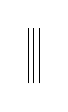
\begin{tikzpicture}\draw (0,0)--(0,.7);\draw (.07,0)--(.07,.7);\draw (.14,0)--(.14,.7);\end{tikzpicture}}
\mspage{45}

\mspage{9}
\[(**)\quad\diagram{\begin{tikzcd}&H^\bullet_{\underline D}(\inserted{\unsure{\overline X|X}},\xi)\arrow[dl,"i^*"']\arrow[dr,"i'^*"]&\\H^\bullet_{\underline D}(U,\xi)\arrow[dr,"i_0'^*"']&&H^\bullet_{\underline D}(U',\xi)\arrow[dl,"i_0^*"]\\&H^\bullet_{\underline D}(U\cap U',\xi)&\end{tikzcd}};\]
\margin{\uline{NB} On a ce carré cartésien, pour $\uline{\forall}\ \xi\in\underline D(\unsure{\overline X|X})$, pas seulement $\xi$ constant\ldots}
Notons pour ceci que si \deleted{\unsure{$\psi$|que}}
\[\psi=\underline k\circ\varphi:\overline X\longrightarrow\Delta^1\times\Delta^1=\underline Q\]
\[\sigma=\underline k_*(\sigma_0)=\underline k_*(\varphi_*(\xi_{\overline X}))=\psi_*(\xi_{\overline X}),\]
d'où
\[H^\bullet_{\underline D}(\Delta^1\times\Delta^1,\sigma)\simeq H^\bullet_{\underline D}(\overline X,\xi)\xrightarrow{\sim}H^\bullet_{\underline D}(X,\xi)\]
\inserted{car $\alpha:X\longrightarrow\overline X$ est $\in W$}
D'autre part, comme $e=(1,1)$ élément final de $\Delta^1\times\Delta^1=\underline Q$ donc $e-\underline Q$ asph.,
\[\deleted{\unsure{\theta}}\qquad\underbrace{H^\bullet_{\underline D}(Q,\sigma)}_{H^\bullet_{\underline D}(\inserted{\unsure{\overline X|X}},\xi)}\simeq\sigma(e)=\sigma(1,1)\deleted{\unsure{\leftarrow\cdots}},\]
d'où l'assertion.
Ça doit faire partie, d'autre part, des propriétés générales des carrés cartésiens \inserted{``dans $\mathcal A$''} (comme (**)), que
\[i_0'^*\text{ iso}\Longleftrightarrow i'^*\text{ iso},\]
\margin{\uuline{à vérifier} (ou à \unsure{mettre en axiome} sur les dérivateurs.)}
\deleted{\unsure{Et}} comme \inserted{ceci} est vrai pour $\uline{\forall}\ \xi\in\mathcal A=\underline De$, cela donne
\[i'_0\in W_{\underline D}\Longrightarrow i'\in W_{\underline D}.\]

